\SourceLeaf{209}\clearpage
\begin{center}
[ZUR THEORIE DER PARALLELLINIEN.]
\end{center}

\begin{center}
[1.]

PARALLELLINIEN.
\end{center}

1. Wenn die Geraden $AM\mathinner{.\,.\,.}$, $BN\mathinner{.\,.\,.}$ einander nicht schneiden, jede
durch $A$ zwischen $AM\mathinner{.\,.\,.}$ und $AB\mathinner{.\,.\,.}$ gelegte Gerade hingegen die $BN\mathinner{.\,.\,.}$ schneidet:
so heisst $AM\mathinner{.\,.\,.}$ mit $BN\mathinner{.\,.\,.}$ parallel.

2. Geht eine Gerade beständig durch
den Punkt $A$, und gelangt durch Drehung aus
der Lage $AB\mathinner{.\,.\,.}$ auf der Seite, wo $BN$ liegt,
zuletzt in die Lage $AC\mathinner{.\,.\,.}$, die der ersten entgegengesetzt ist, so ist sie anfangs schneidend,
zuletzt nicht schneidend, also muss es gewiss
Eine und nur Eine Lage geben, die die Scheidung der schneidenden und nicht
schneidenden [Geraden] ist, und zwar wird diess die erste nicht schneidende sein,
also nach unserer Definition die Parallele $AM\mathinner{.\,.\,.}$, da es offenbar keine letzte
schneidende geben kann.

\begin{center}
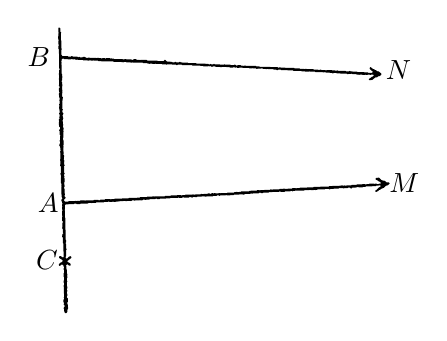
\begin{tikzpicture}[x=0.00516899cm,y=-0.00516899cm]
\fill[even odd rule] (94,22) -- (94,32) -- (95,34) -- (94,35) -- (94,42) -- (93,43) -- (93,47) -- (94,48) -- (94,51) -- (95,52) -- (94,54) -- (94,62) -- (95,63) -- (95,65) -- (94,66) -- (94,73) -- (95,74) -- (95,84) -- (96,85) -- (96,121) -- (97,122) -- (97,124) -- (96,125) -- (96,132) -- (95,133) -- (95,137) -- (96,138) -- (96,145) -- (95,146) -- (95,148) -- (96,149) -- (96,161) -- (95,163) -- (97,166) -- (97,168) -- (95,171) -- (95,175) -- (96,176) -- (96,179) -- (97,180) -- (97,181) -- (95,183) -- (95,186) -- (96,187) -- (96,192) -- (97,193) -- (97,198) -- (96,199) -- (97,201) -- (97,208) -- (96,209) -- (96,212) -- (97,213) -- (96,215) -- (96,220) -- (97,221) -- (96,223) -- (97,225) -- (97,230) -- (96,231) -- (96,233) -- (97,234) -- (97,239) -- (96,241) -- (97,242) -- (97,244) -- (95,246) -- (95,249) -- (96,250) -- (96,252) -- (95,253) -- (95,260) -- (96,261) -- (96,264) -- (98,266) -- (98,270) -- (96,272) -- (96,274) -- (97,275) -- (97,283) -- (99,286) -- (98,288) -- (98,297) -- (97,298) -- (97,300) -- (98,301) -- (98,305) -- (97,306) -- (96,310) -- (98,313) -- (98,315) -- (99,316) -- (99,321) -- (100,322) -- (98,326) -- (99,328) -- (99,344) -- (98,345) -- (98,347) -- (99,348) -- (99,357) -- (98,358) -- (98,360) -- (100,362) -- (100,378) -- (99,379) -- (99,381) -- (100,382) -- (100,386) -- (101,387) -- (100,389) -- (100,402) -- (102,405) -- (101,407) -- (101,410) -- (102,411) -- (101,413) -- (101,430) -- (102,431) -- (102,436) -- (104,441) -- (101,444) -- (101,446) -- (103,448) -- (103,451) -- (104,452) -- (104,454) -- (103,455) -- (103,459) -- (104,460) -- (103,462) -- (103,467) -- (104,468) -- (104,471) -- (103,472) -- (103,482) -- (104,483) -- (104,485) -- (103,486) -- (103,495) -- (105,497) -- (105,499) -- (104,500) -- (104,511) -- (103,513) -- (105,516) -- (105,524) -- (106,525) -- (106,526) -- (104,528) -- (103,534) -- (105,537) -- (105,550) -- (106,551) -- (106,570) -- (107,571) -- (107,584) -- (106,585) -- (104,585) -- (100,582) -- (97,582) -- (96,583) -- (96,586) -- (98,588) -- (102,590) -- (105,593) -- (105,594) -- (102,597) -- (99,598) -- (95,602) -- (95,604) -- (97,606) -- (98,606) -- (101,603) -- (104,603) -- (107,606) -- (107,608) -- (108,609) -- (108,611) -- (107,612) -- (107,615) -- (108,616) -- (108,623) -- (107,624) -- (107,633) -- (108,634) -- (108,641) -- (107,642) -- (107,647) -- (108,648) -- (108,653) -- (107,654) -- (108,682) -- (107,684) -- (108,685) -- (108,687) -- (106,690) -- (106,694) -- (108,697) -- (107,701) -- (109,703) -- (109,706) -- (107,709) -- (107,711) -- (108,712) -- (108,717) -- (109,718) -- (109,720) -- (111,722) -- (113,722) -- (115,720) -- (116,718) -- (116,714) -- (118,710) -- (118,708) -- (117,707) -- (117,701) -- (116,700) -- (116,695) -- (117,694) -- (117,686) -- (115,684) -- (115,680) -- (116,679) -- (116,675) -- (115,674) -- (115,669) -- (116,668) -- (116,666) -- (115,665) -- (115,662) -- (116,661) -- (116,657) -- (115,656) -- (115,645) -- (116,644) -- (115,642) -- (115,636) -- (116,635) -- (116,632) -- (115,630) -- (116,629) -- (116,626) -- (115,625) -- (115,616) -- (114,615) -- (113,604) -- (115,602) -- (118,603) -- (120,605) -- (123,605) -- (124,604) -- (124,601) -- (122,599) -- (118,597) -- (116,595) -- (116,594) -- (126,586) -- (126,584) -- (124,582) -- (120,583) -- (115,588) -- (114,588) -- (112,586) -- (112,583) -- (113,582) -- (113,567) -- (114,566) -- (114,564) -- (113,563) -- (113,552) -- (112,551) -- (112,549) -- (113,548) -- (113,543) -- (112,542) -- (112,518) -- (111,517) -- (111,488) -- (110,487) -- (110,470) -- (109,469) -- (110,467) -- (110,457) -- (112,455) -- (118,455) -- (119,454) -- (132,454) -- (133,453) -- (138,453) -- (139,454) -- (147,454) -- (148,453) -- (165,453) -- (169,451) -- (174,451) -- (176,452) -- (177,451) -- (186,451) -- (187,450) -- (205,450) -- (206,449) -- (215,449) -- (216,448) -- (219,448) -- (220,449) -- (226,449) -- (227,448) -- (234,449) -- (235,448) -- (239,448) -- (240,447) -- (243,448) -- (244,447) -- (253,447) -- (254,446) -- (258,446) -- (259,447) -- (262,447) -- (263,446) -- (270,446) -- (272,447) -- (275,445) -- (280,445) -- (281,446) -- (283,445) -- (293,445) -- (294,444) -- (296,445) -- (300,445) -- (302,443) -- (306,443) -- (307,444) -- (309,444) -- (310,443) -- (317,443) -- (318,442) -- (332,442) -- (333,441) -- (336,441) -- (337,442) -- (342,442) -- (343,441) -- (357,441) -- (358,440) -- (368,440) -- (369,439) -- (387,439) -- (388,438) -- (390,438) -- (391,439) -- (397,439) -- (400,437) -- (402,438) -- (414,438) -- (415,437) -- (420,437) -- (421,438) -- (423,438) -- (427,436) -- (429,437) -- (434,437) -- (435,436) -- (445,436) -- (446,435) -- (453,435) -- (454,436) -- (457,436) -- (458,435) -- (473,435) -- (474,434) -- (482,434) -- (483,433) -- (488,433) -- (490,434) -- (491,433) -- (504,433) -- (505,432) -- (507,432) -- (508,433) -- (515,433) -- (516,432) -- (524,432) -- (525,431) -- (537,431) -- (538,430) -- (546,430) -- (547,431) -- (549,431) -- (553,429) -- (565,429) -- (566,428) -- (568,428) -- (569,429) -- (571,428) -- (585,428) -- (588,426) -- (590,426) -- (591,427) -- (596,427) -- (597,426) -- (610,426) -- (611,425) -- (619,425) -- (620,424) -- (636,424) -- (637,423) -- (639,423) -- (640,424) -- (649,424) -- (650,423) -- (663,423) -- (664,422) -- (668,422) -- (669,423) -- (670,422) -- (674,422) -- (675,421) -- (697,421) -- (698,420) -- (710,420) -- (711,419) -- (713,419) -- (714,420) -- (720,420) -- (721,419) -- (723,419) -- (725,420) -- (726,419) -- (729,419) -- (730,418) -- (748,418) -- (749,417) -- (758,417) -- (759,418) -- (761,418) -- (762,417) -- (769,417) -- (770,416) -- (782,416) -- (783,415) -- (793,415) -- (795,416) -- (796,415) -- (804,415) -- (805,414) -- (810,414) -- (812,416) -- (813,416) -- (815,414) -- (823,414) -- (824,413) -- (827,413) -- (828,412) -- (830,412) -- (831,413) -- (841,413) -- (842,412) -- (847,412) -- (848,411) -- (873,410) -- (874,409) -- (880,409) -- (881,408) -- (884,408) -- (885,409) -- (885,411) -- (880,414) -- (874,420) -- (872,421) -- (872,423) -- (873,424) -- (875,424) -- (876,423) -- (878,423) -- (882,419) -- (884,419) -- (886,417) -- (893,414) -- (898,409) -- (903,408) -- (907,404) -- (907,403) -- (905,401) -- (900,401) -- (895,397) -- (889,396) -- (887,395) -- (881,389) -- (879,389) -- (878,390) -- (874,390) -- (873,391) -- (873,394) -- (879,397) -- (881,399) -- (883,399) -- (886,402) -- (885,404) -- (881,404) -- (880,405) -- (876,405) -- (875,404) -- (871,404) -- (870,405) -- (868,404) -- (858,404) -- (857,405) -- (851,405) -- (850,406) -- (847,406) -- (846,405) -- (841,405) -- (840,406) -- (827,406) -- (826,407) -- (814,407) -- (813,408) -- (802,408) -- (801,409) -- (798,409) -- (797,408) -- (795,409) -- (789,408) -- (788,409) -- (759,410) -- (758,411) -- (738,411) -- (737,412) -- (721,412) -- (720,413) -- (705,413) -- (704,414) -- (687,414) -- (686,415) -- (679,415) -- (678,416) -- (676,415) -- (669,415) -- (668,416) -- (658,416) -- (657,417) -- (650,417) -- (649,416) -- (647,416) -- (646,417) -- (637,417) -- (636,418) -- (621,418) -- (620,419) -- (615,418) -- (614,419) -- (600,419) -- (599,420) -- (590,420) -- (589,421) -- (587,420) -- (582,420) -- (581,421) -- (567,421) -- (566,422) -- (563,422) -- (562,423) -- (543,423) -- (542,424) -- (538,424) -- (537,425) -- (530,424) -- (529,425) -- (526,425) -- (525,426) -- (509,426) -- (508,427) -- (494,427) -- (493,428) -- (491,427) -- (488,427) -- (487,428) -- (480,428) -- (479,427) -- (474,428) -- (472,427) -- (468,429) -- (466,429) -- (465,428) -- (461,428) -- (460,429) -- (451,429) -- (450,430) -- (444,429) -- (443,430) -- (431,430) -- (430,431) -- (426,431) -- (425,430) -- (423,431) -- (406,431) -- (405,432) -- (399,432) -- (398,433) -- (395,433) -- (394,432) -- (386,432) -- (385,433) -- (370,433) -- (369,434) -- (356,434) -- (355,435) -- (331,435) -- (330,436) -- (328,435) -- (325,435) -- (324,436) -- (312,436) -- (311,437) -- (295,437) -- (294,438) -- (288,438) -- (287,439) -- (267,439) -- (266,440) -- (251,440) -- (250,441) -- (232,441) -- (231,442) -- (224,442) -- (223,443) -- (221,442) -- (209,442) -- (208,443) -- (198,443) -- (195,445) -- (193,445) -- (192,444) -- (181,444) -- (180,445) -- (161,445) -- (160,446) -- (158,445) -- (148,445) -- (147,446) -- (140,446) -- (139,447) -- (135,446) -- (134,447) -- (119,447) -- (118,448) -- (110,448) -- (108,446) -- (108,443) -- (112,439) -- (112,438) -- (109,435) -- (110,429) -- (109,428) -- (109,417) -- (108,416) -- (108,412) -- (109,411) -- (109,408) -- (108,407) -- (109,405) -- (108,403) -- (108,401) -- (109,400) -- (109,391) -- (108,390) -- (109,386) -- (108,385) -- (108,381) -- (109,380) -- (109,378) -- (108,377) -- (108,364) -- (107,362) -- (109,360) -- (109,358) -- (108,357) -- (108,350) -- (109,348) -- (107,346) -- (108,335) -- (106,332) -- (107,330) -- (107,326) -- (106,325) -- (106,315) -- (107,314) -- (106,312) -- (106,309) -- (107,308) -- (107,299) -- (106,298) -- (105,292) -- (106,291) -- (106,277) -- (107,276) -- (106,274) -- (106,271) -- (107,270) -- (107,268) -- (105,265) -- (106,259) -- (105,258) -- (105,252) -- (104,251) -- (105,245) -- (106,244) -- (104,236) -- (106,233) -- (106,231) -- (104,229) -- (104,224) -- (105,222) -- (103,220) -- (104,218) -- (104,203) -- (103,201) -- (104,200) -- (105,192) -- (103,190) -- (103,182) -- (104,181) -- (104,179) -- (103,178) -- (104,176) -- (104,174) -- (103,173) -- (103,165) -- (104,164) -- (104,161) -- (103,160) -- (103,155) -- (102,154) -- (102,151) -- (103,150) -- (103,144) -- (104,143) -- (104,141) -- (103,140) -- (103,135) -- (102,134) -- (102,112) -- (101,111) -- (101,109) -- (102,108) -- (101,103) -- (102,102) -- (102,99) -- (104,97) -- (107,97) -- (108,98) -- (117,98) -- (118,99) -- (124,99) -- (125,98) -- (132,99) -- (134,98) -- (137,100) -- (141,99) -- (142,100) -- (154,100) -- (155,101) -- (165,101) -- (166,102) -- (169,102) -- (170,101) -- (173,101) -- (174,102) -- (179,102) -- (181,101) -- (182,102) -- (191,102) -- (192,103) -- (199,103) -- (200,104) -- (229,104) -- (230,105) -- (249,105) -- (250,106) -- (252,105) -- (254,106) -- (256,105) -- (260,105) -- (261,106) -- (271,106) -- (272,107) -- (274,107) -- (275,106) -- (277,107) -- (301,107) -- (302,108) -- (312,108) -- (313,109) -- (317,109) -- (318,110) -- (320,109) -- (324,109) -- (325,110) -- (330,110) -- (332,109) -- (333,110) -- (348,110) -- (349,111) -- (358,111) -- (359,112) -- (361,111) -- (373,111) -- (374,112) -- (383,112) -- (384,113) -- (386,113) -- (387,112) -- (397,112) -- (398,113) -- (422,113) -- (423,114) -- (442,114) -- (443,115) -- (449,115) -- (450,116) -- (461,116) -- (462,115) -- (466,116) -- (468,115) -- (470,117) -- (472,117) -- (473,116) -- (479,116) -- (480,117) -- (490,117) -- (491,118) -- (495,118) -- (496,117) -- (506,117) -- (507,118) -- (514,118) -- (515,119) -- (522,119) -- (523,118) -- (529,119) -- (531,118) -- (534,120) -- (537,120) -- (538,119) -- (546,119) -- (547,120) -- (562,120) -- (563,121) -- (569,121) -- (571,120) -- (572,121) -- (579,121) -- (580,122) -- (595,121) -- (596,122) -- (602,122) -- (603,123) -- (605,123) -- (606,122) -- (608,122) -- (609,123) -- (622,123) -- (623,124) -- (629,124) -- (630,125) -- (633,125) -- (634,124) -- (640,124) -- (641,125) -- (656,125) -- (657,126) -- (670,126) -- (671,127) -- (690,127) -- (691,128) -- (699,128) -- (700,129) -- (708,129) -- (710,128) -- (711,129) -- (724,129) -- (725,130) -- (743,130) -- (744,131) -- (749,130) -- (750,131) -- (766,132) -- (767,133) -- (769,133) -- (770,132) -- (776,132) -- (777,133) -- (786,133) -- (787,134) -- (802,134) -- (803,135) -- (815,134) -- (816,135) -- (825,135) -- (826,136) -- (831,136) -- (832,137) -- (834,136) -- (840,136) -- (841,137) -- (846,137) -- (847,136) -- (849,137) -- (853,137) -- (854,136) -- (858,136) -- (859,137) -- (861,137) -- (862,136) -- (867,136) -- (868,137) -- (868,139) -- (866,141) -- (864,141) -- (861,144) -- (860,144) -- (856,148) -- (857,150) -- (862,150) -- (863,149) -- (865,149) -- (871,144) -- (873,143) -- (876,143) -- (880,140) -- (883,140) -- (887,136) -- (887,134) -- (880,128) -- (877,128) -- (873,125) -- (871,125) -- (869,123) -- (867,123) -- (861,118) -- (860,118) -- (858,120) -- (859,123) -- (866,129) -- (866,130) -- (864,132) -- (855,132) -- (854,131) -- (845,131) -- (844,130) -- (828,130) -- (827,129) -- (816,129) -- (815,128) -- (811,128) -- (810,127) -- (808,128) -- (800,128) -- (799,127) -- (781,127) -- (780,126) -- (774,127) -- (773,126) -- (766,126) -- (765,125) -- (753,125) -- (752,126) -- (750,126) -- (749,125) -- (740,125) -- (739,124) -- (732,125) -- (731,124) -- (721,124) -- (720,123) -- (704,123) -- (703,122) -- (700,122) -- (698,123) -- (697,122) -- (687,122) -- (686,121) -- (674,121) -- (673,120) -- (651,120) -- (650,119) -- (639,119) -- (638,118) -- (636,119) -- (633,119) -- (632,118) -- (615,118) -- (614,117) -- (588,117) -- (587,116) -- (580,116) -- (579,115) -- (555,115) -- (554,114) -- (550,114) -- (549,115) -- (547,115) -- (546,114) -- (542,114) -- (541,113) -- (534,113) -- (533,114) -- (531,114) -- (528,112) -- (526,112) -- (525,113) -- (517,113) -- (516,112) -- (503,112) -- (502,111) -- (500,112) -- (491,112) -- (490,111) -- (478,111) -- (477,110) -- (475,110) -- (474,111) -- (469,111) -- (468,110) -- (466,111) -- (463,111) -- (462,110) -- (455,110) -- (454,109) -- (433,109) -- (432,108) -- (413,108) -- (412,107) -- (398,107) -- (397,106) -- (394,106) -- (393,105) -- (391,105) -- (390,106) -- (383,106) -- (382,105) -- (380,105) -- (379,106) -- (374,106) -- (373,105) -- (360,104) -- (356,100) -- (354,100) -- (354,101) -- (352,103) -- (338,103) -- (337,102) -- (313,102) -- (310,100) -- (296,100) -- (294,101) -- (293,100) -- (287,100) -- (283,98) -- (280,98) -- (277,100) -- (274,100) -- (273,99) -- (261,99) -- (260,98) -- (257,98) -- (256,99) -- (252,99) -- (251,98) -- (231,98) -- (230,97) -- (225,97) -- (224,96) -- (222,97) -- (220,96) -- (211,96) -- (210,97) -- (208,96) -- (202,96) -- (200,97) -- (199,96) -- (194,96) -- (193,95) -- (188,95) -- (187,96) -- (185,95) -- (170,95) -- (169,94) -- (167,95) -- (162,95) -- (159,93) -- (154,93) -- (153,94) -- (147,94) -- (146,93) -- (144,93) -- (142,94) -- (140,92) -- (129,92) -- (128,91) -- (126,91) -- (125,92) -- (118,92) -- (117,91) -- (104,91) -- (101,87) -- (101,76) -- (102,75) -- (102,72) -- (101,71) -- (101,53) -- (100,52) -- (100,35) -- (101,33) -- (99,31) -- (99,23) -- (97,21) -- (95,21) -- cycle;
\node[inner sep=0pt] at (46,94) {$B$};
\node[inner sep=0pt] at (929,126) {$N$};
\node[inner sep=0pt] at (943,402) {$M$};
\node[inner sep=0pt] at (69,452) {$A$};
\node[inner sep=0pt] at (66,591) {$C$};
\end{tikzpicture}

\end{center}

3. In unserer Definition sind in beiden Linien bestimmte Anfangspunkte
$A, B$ vorausgesetzt. Man sieht aber leicht, dass der Parallelismus davon unabhängig ist, in so fern nur der Sinn der Richtungen, nach welchen die Linien
als unbegrenzt betrachtet werden, derselbe bleibt. Nimmt man nemlich statt
$B$ einen andern Anfangspunkt $B'$, sei es auf der Linie $BN\mathinner{.\,.\,.}$, oder wo immer
